\documentclass{standalone}
\usepackage{tikz,pgfplots,calc}
\usetikzlibrary{positioning,calc}
\usetikzlibrary{arrows}
\usepackage{tkz-euclide}
\usetkzobj{all}


\renewcommand{\familydefault}{\sfdefault}

\tikzset{
  mynode/.style = {draw, minimum width = .4cm, minimum height = 2cm}}

\begin{document}
\begin{tikzpicture}[>=stealth', thick]
    \node (m1) at (0, 0) {
\includegraphics{m1.png}};
    \node (m2) [right=of m1] {
\includegraphics{m2.png}};
    \node (t1) [below=5pt of m2, scale = 3] {Men};
    \node (m3) [right=of m2] {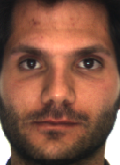
\includegraphics{m3.png}};

    \node (w1) [anchor = west, right=4cm of m3] {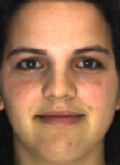
\includegraphics{w1.png}};
    \node (w2) [right=of w1] {
\includegraphics{w2.png}};
    \node (t2) [below=5pt of w2, scale = 3] {Women};
    \node (w3) [right=of w2] {
\includegraphics{w3.png}};
\end{tikzpicture}
\end{document}